\section*{Questão 1}

\paragraph{}Para o conjunto de dados da tabela 1 deseja-se
calcular os ajustes polinomiais de ordem 1,2,3,5 e 10.
 Ou seja, achar quais são os polinômios de ordem n $y_{n}(t)$ 
\begin{displaymath}
y_n(t) = \alpha_{0}n^{0} + \alpha_{1}n^{1} + \ldots 
									\alpha_{n}t^{n}
\end{displaymath}
que 
miniminizam o erro quadrático médio 
\begin{equation}
e_{n} = \sqrt{\sum _{i = 1}^{m} [y_{i} - y_{n}(t_{i})]^2}
\label{eq:erro}
\end{equation}

sobre o conjunto de m dados na forma $(t_{i}, y_{i})$. 
A tabela apresenta 17 desses pares, nesse caso m = 17. 
A função PolynomialFitting do anexo realiza o cálculo dos 
coeficientes e os resultados são plotados nos gráficos 
\ref{fig:quest1-a} e \ref{fig:quest1-b}. No primeiro gráfico
vemos os ajustes para n = 1,2 e 3. No segundo vemos n = 5 e 10.
Os resultados foram separados em dois gráficos para permitir 
melhor visualização das curvas. As tabelas de \ref{tab:quest1-X1} 
a \ref{tab:quest1-X10} mostram os coeficientes $\alpha_n$ calculados.

\paragraph{}Descrevemos brevemente o algoritmo utilizado.
Considere a expressão $[y_{i} - y_{n}(t_{i})]$. Pela fórmula
\ref{eq:erro} vemos que $e_n$ será mínimo quando essa expressão
for mínima, i.e.:$y_{i} = y_{n}(t_{i}), \forall 
t = \{ 1, 2, \ldots, m \}$, onde n é a ordem dada do polinômio  e m o número
de dados tomados. As incógnitas desse problema são os coeficientes $\alpha_j$,
com $j = {0, 1, \ldots, n}$. Esse sistema pode ser reescrito na forma $Ax = y$
com:

\begin{minipage}{0.3\textwidth}
\begin{displaymath}
	A_{\mbox{mx(n+1)}} = \left(
	\begin{array}{lllll}
	1 & t_1 & t_1^2 & \ldots & t_1^n \\
	1 & t_2 & t_2^2 & \ldots & t_2^n \\
	\vdots & \vdots & \vdots &\ddots  & \vdots \\
	1 & t_m & t_m^2 & \ldots & t_m^n \\
	\end{array}\right)
\end{displaymath}
\end{minipage}
\hspace{2 cm}
\begin{minipage}{0.3\textwidth}
\begin{displaymath}
	x_{\mbox{(n+1)x1}} = \left(
	\begin{array}{l}
	\alpha_0 \\
	\alpha_1 \\
	\vdots \\
	\alpha_n \\
	\end{array}\right)
\end{displaymath}
\end{minipage}
\begin{minipage}{0.3\textwidth}
\begin{displaymath}
	y_{\mbox{mx1}} = \left(
	\begin{array}{l}
	y_0 \\
	y_1 \\
	\vdots \\
	y_n \\
	\end{array}\right)
\end{displaymath}
\end{minipage}

\paragraph{}O sistema pode ser resolvido de diversas formas. Se quisermos
inverter matrizes podemos usar:

\begin{equation}
	x = (A^T A)^{-1}A^T y
	\label{eq:SolvingSystemGeral}
\end{equation}

\paragraph{} Podemos também usar as diversas técnicas de solução de sistemas
estudadas ao longo do curso. Para isso fazemos $D =A^T A$ e $E=(A^T y)$ e podemos
usar os métodos de Jacobi ou Gauss-Seidel por exemplo para resolver $Dx = E$

\paragraph{}Na equação \ref{eq:SolvingSystemGeral} a existência da inversa 
$(A^T A)^{-1}$ se baseia no fato de que a matriz A tem colunas linearmente
independentes, o que é garantido no caso em que existem ao menos 2 $t_i$'s 
diferentes entre si.

\paragraph{} No caso em que m = n+1 teremos a matriz A quadrada e o
erro dever ser zero. Isto é, o polinômio coincide perfeitamente com os dados
nos pontos tomados. Nesse caso temos o polinômio interpolador. Nos outros casos
a interpolação não é perfeita e temos apenas o polinômio de ordem n que melhor
se ajusta aos dados.

\paragraph{}Em nosso código o sistema é resolvido pela inversão de matrizes. 
A rotina foi implementada em C e o anexo contém todos os algoritmo usados,
inclusive os de interseção de matrizes,  multiplicação, soma e transposição.
Essas rotinas são consideradas auxiliares e portanto apresentadas separadamente
dos códigos principais para interpolação. 

\paragraph{}Os gráficos \ref{fig:quest1-a} e \ref{fig:quest1-b} nos mostram
 que a medida que aumenta a ordem n
do polinômio temos mais oscilações no fitting. Sem saber o que os dados
representam e para que serão usados é difícil decidir sobre qual o ajuste
mais adequado. Sem essa informação podemos apenas qualificar os ajustes quanto
aos erros quadráticos médios que deram origem ao método que
calculou as interpolações. A expressão \ref{eq:erro} pode ser 
calucalada para cada uma das curvas. Os resultados são apresentados na tabela
a seguir.

\begin{table}[!htp]
\centering
	\begin{tabular}{|l|l|}\hline
	n & $E_{n}$ \\ \hline
	 1	& 4.967 \\ \hline	
	 2	& 5.045\\ \hline	
	 3	& 5.861\\ \hline	
	 5	& 6.126\\ \hline	
	10	& 7.616\\ \hline	
	\end{tabular}
	\caption{Erro quadrático médio para n = 1,2,3,5 e 10}
	\label{tab:ERMS-quest1}
\end{table}

\paragraph{}Vemos que nesse caso aumentar o grau do polinômio de
interpolação nos deu um maior erro quadrático médio. Baseado nesses
dados podemos dizer que o melhor ajuste dentre esses 5 feitos é o 
de primeira ordem. 

\FloatBarrier
\begin{figure}[!htp]
	\begin{subfigure}[!htp]{0.5\textwidth}
	% GNUPLOT: LaTeX picture with Postscript
\begingroup
  \fontfamily{phv}%
  \selectfont
\definecolor{t}{rgb}{0.5,0.5,0.5}
  \makeatletter
  \providecommand\color[2][]{%
    \GenericError{(gnuplot) \space\space\space\@spaces}{%
      Package color not loaded in conjunction with
      terminal option `colourtext'%
    }{See the gnuplot documentation for explanation.%
    }{Either use 'blacktext' in gnuplot or load the package
      color.sty in LaTeX.}%
    \renewcommand\color[2][]{}%
  }%
  \providecommand\includegraphics[2][]{%
    \GenericError{(gnuplot) \space\space\space\@spaces}{%
      Package graphicx or graphics not loaded%
    }{See the gnuplot documentation for explanation.%
    }{The gnuplot epslatex terminal needs graphicx.sty or graphics.sty.}%
    \renewcommand\includegraphics[2][]{}%
  }%
  \providecommand\rotatebox[2]{#2}%
  \@ifundefined{ifGPcolor}{%
    \newif\ifGPcolor
    \GPcolortrue
  }{}%
  \@ifundefined{ifGPblacktext}{%
    \newif\ifGPblacktext
    \GPblacktextfalse
  }{}%
  % define a \g@addto@macro without @ in the name:
  \let\gplgaddtomacro\g@addto@macro
  % define empty templates for all commands taking text:
  \gdef\gplbacktext{}%
  \gdef\gplfronttext{}%
  \makeatother
  \ifGPblacktext
    % no textcolor at all
    \def\colorrgb#1{}%
    \def\colorgray#1{}%
  \else
    % gray or color?
    \ifGPcolor
      \def\colorrgb#1{\color[rgb]{#1}}%
      \def\colorgray#1{\color[gray]{#1}}%
      \expandafter\def\csname LTw\endcsname{\color{white}}%
      \expandafter\def\csname LTb\endcsname{\color{black}}%
      \expandafter\def\csname LTa\endcsname{\color{black}}%
      \expandafter\def\csname LT0\endcsname{\color[rgb]{1,0,0}}%
      \expandafter\def\csname LT1\endcsname{\color[rgb]{0,1,0}}%
      \expandafter\def\csname LT2\endcsname{\color[rgb]{0,0,1}}%
      \expandafter\def\csname LT3\endcsname{\color[rgb]{1,0,1}}%
      \expandafter\def\csname LT4\endcsname{\color[rgb]{0,1,1}}%
      \expandafter\def\csname LT5\endcsname{\color[rgb]{1,1,0}}%
      \expandafter\def\csname LT6\endcsname{\color[rgb]{0,0,0}}%
      \expandafter\def\csname LT7\endcsname{\color[rgb]{1,0.3,0}}%
      \expandafter\def\csname LT8\endcsname{\color[rgb]{0.5,0.5,0.5}}%
    \else
      % gray
      \def\colorrgb#1{\color{black}}%
      \def\colorgray#1{\color[gray]{#1}}%
      \expandafter\def\csname LTw\endcsname{\color{white}}%
      \expandafter\def\csname LTb\endcsname{\color{black}}%
      \expandafter\def\csname LTa\endcsname{\color{black}}%
      \expandafter\def\csname LT0\endcsname{\color{black}}%
      \expandafter\def\csname LT1\endcsname{\color{black}}%
      \expandafter\def\csname LT2\endcsname{\color{black}}%
      \expandafter\def\csname LT3\endcsname{\color{black}}%
      \expandafter\def\csname LT4\endcsname{\color{black}}%
      \expandafter\def\csname LT5\endcsname{\color{black}}%
      \expandafter\def\csname LT6\endcsname{\color{black}}%
      \expandafter\def\csname LT7\endcsname{\color{black}}%
      \expandafter\def\csname LT8\endcsname{\color{black}}%
    \fi
  \fi
  \setlength{\unitlength}{0.0500bp}%
  \begin{picture}(7936.00,5668.00)%
    \gplgaddtomacro\gplbacktext{%
      \csname LTb\endcsname%
      \put(558,1476){\makebox(0,0)[r]{\strut{} 0}}%
      \put(558,1882){\makebox(0,0)[r]{\strut{} 1}}%
      \put(558,2287){\makebox(0,0)[r]{\strut{} 2}}%
      \put(558,2693){\makebox(0,0)[r]{\strut{} 3}}%
      \put(558,3099){\makebox(0,0)[r]{\strut{} 4}}%
      \put(558,3504){\makebox(0,0)[r]{\strut{} 5}}%
      \put(558,3910){\makebox(0,0)[r]{\strut{} 6}}%
      \put(558,4316){\makebox(0,0)[r]{\strut{} 7}}%
      \put(558,4721){\makebox(0,0)[r]{\strut{} 8}}%
      \put(558,5127){\makebox(0,0)[r]{\strut{} 9}}%
      \put(666,1296){\makebox(0,0){\strut{} 0}}%
      \put(1438,1296){\makebox(0,0){\strut{} 0.2}}%
      \put(2209,1296){\makebox(0,0){\strut{} 0.4}}%
      \put(2981,1296){\makebox(0,0){\strut{} 0.6}}%
      \put(3753,1296){\makebox(0,0){\strut{} 0.8}}%
      \put(4524,1296){\makebox(0,0){\strut{} 1}}%
      \put(5296,1296){\makebox(0,0){\strut{} 1.2}}%
      \put(6068,1296){\makebox(0,0){\strut{} 1.4}}%
      \put(6839,1296){\makebox(0,0){\strut{} 1.6}}%
      \put(7611,1296){\makebox(0,0){\strut{} 1.8}}%
      \put(144,3301){\makebox(0,0){\strut{}y(t)}}%
      \put(4138,1026){\makebox(0,0){\strut{}t}}%
      \put(4138,5397){\makebox(0,0){\strut{}Ajuste Polinomial}}%
    }%
    \gplgaddtomacro\gplfronttext{%
      \csname LTb\endcsname%
      \put(4377,693){\makebox(0,0)[r]{\strut{}$y_{1}(t)$}}%
      \csname LTb\endcsname%
      \put(4377,513){\makebox(0,0)[r]{\strut{}$y_{2}(t)$}}%
      \csname LTb\endcsname%
      \put(4377,333){\makebox(0,0)[r]{\strut{}$y_{3}(t)$}}%
      \csname LTb\endcsname%
      \put(4377,153){\makebox(0,0)[r]{\strut{}data points}}%
    }%
    \gplbacktext
    \put(0,0){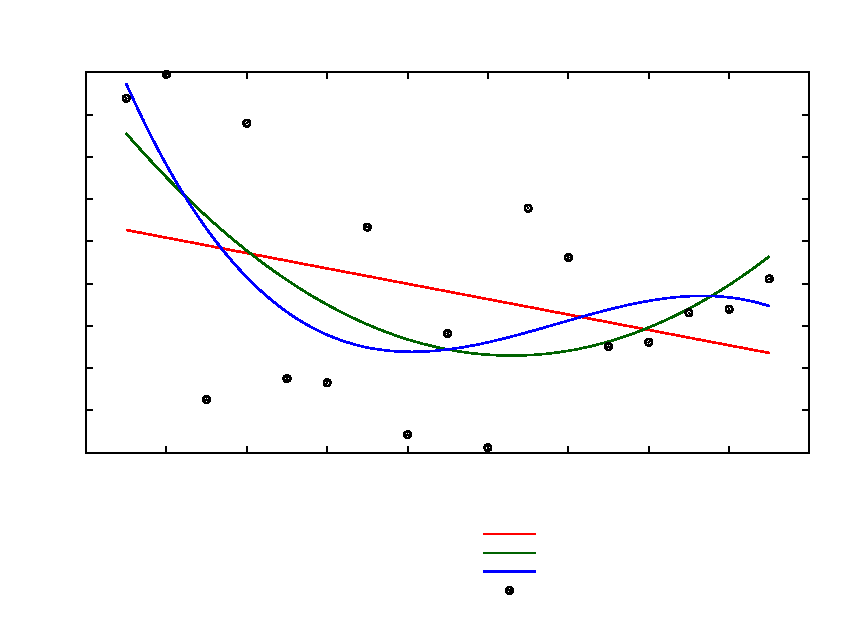
\includegraphics{./../LaTeX/graph/quest1-a}}%
    \gplfronttext
  \end{picture}%
\endgroup

	\caption{Fitting para n = 1,2 e 3}
	\label{fig:quest1-a}
	\end{subfigure}

	\begin{subfigure}[!htp]{0.5\textwidth}
	% GNUPLOT: LaTeX picture with Postscript
\begingroup
  \fontfamily{phv}%
  \selectfont
\definecolor{t}{rgb}{0.5,0.5,0.5}
  \makeatletter
  \providecommand\color[2][]{%
    \GenericError{(gnuplot) \space\space\space\@spaces}{%
      Package color not loaded in conjunction with
      terminal option `colourtext'%
    }{See the gnuplot documentation for explanation.%
    }{Either use 'blacktext' in gnuplot or load the package
      color.sty in LaTeX.}%
    \renewcommand\color[2][]{}%
  }%
  \providecommand\includegraphics[2][]{%
    \GenericError{(gnuplot) \space\space\space\@spaces}{%
      Package graphicx or graphics not loaded%
    }{See the gnuplot documentation for explanation.%
    }{The gnuplot epslatex terminal needs graphicx.sty or graphics.sty.}%
    \renewcommand\includegraphics[2][]{}%
  }%
  \providecommand\rotatebox[2]{#2}%
  \@ifundefined{ifGPcolor}{%
    \newif\ifGPcolor
    \GPcolortrue
  }{}%
  \@ifundefined{ifGPblacktext}{%
    \newif\ifGPblacktext
    \GPblacktextfalse
  }{}%
  % define a \g@addto@macro without @ in the name:
  \let\gplgaddtomacro\g@addto@macro
  % define empty templates for all commands taking text:
  \gdef\gplbacktext{}%
  \gdef\gplfronttext{}%
  \makeatother
  \ifGPblacktext
    % no textcolor at all
    \def\colorrgb#1{}%
    \def\colorgray#1{}%
  \else
    % gray or color?
    \ifGPcolor
      \def\colorrgb#1{\color[rgb]{#1}}%
      \def\colorgray#1{\color[gray]{#1}}%
      \expandafter\def\csname LTw\endcsname{\color{white}}%
      \expandafter\def\csname LTb\endcsname{\color{black}}%
      \expandafter\def\csname LTa\endcsname{\color{black}}%
      \expandafter\def\csname LT0\endcsname{\color[rgb]{1,0,0}}%
      \expandafter\def\csname LT1\endcsname{\color[rgb]{0,1,0}}%
      \expandafter\def\csname LT2\endcsname{\color[rgb]{0,0,1}}%
      \expandafter\def\csname LT3\endcsname{\color[rgb]{1,0,1}}%
      \expandafter\def\csname LT4\endcsname{\color[rgb]{0,1,1}}%
      \expandafter\def\csname LT5\endcsname{\color[rgb]{1,1,0}}%
      \expandafter\def\csname LT6\endcsname{\color[rgb]{0,0,0}}%
      \expandafter\def\csname LT7\endcsname{\color[rgb]{1,0.3,0}}%
      \expandafter\def\csname LT8\endcsname{\color[rgb]{0.5,0.5,0.5}}%
    \else
      % gray
      \def\colorrgb#1{\color{black}}%
      \def\colorgray#1{\color[gray]{#1}}%
      \expandafter\def\csname LTw\endcsname{\color{white}}%
      \expandafter\def\csname LTb\endcsname{\color{black}}%
      \expandafter\def\csname LTa\endcsname{\color{black}}%
      \expandafter\def\csname LT0\endcsname{\color{black}}%
      \expandafter\def\csname LT1\endcsname{\color{black}}%
      \expandafter\def\csname LT2\endcsname{\color{black}}%
      \expandafter\def\csname LT3\endcsname{\color{black}}%
      \expandafter\def\csname LT4\endcsname{\color{black}}%
      \expandafter\def\csname LT5\endcsname{\color{black}}%
      \expandafter\def\csname LT6\endcsname{\color{black}}%
      \expandafter\def\csname LT7\endcsname{\color{black}}%
      \expandafter\def\csname LT8\endcsname{\color{black}}%
    \fi
  \fi
  \setlength{\unitlength}{0.0500bp}%
  \begin{picture}(7936.00,5668.00)%
    \gplgaddtomacro\gplbacktext{%
      \csname LTb\endcsname%
      \put(666,1296){\makebox(0,0)[r]{\strut{} 0}}%
      \put(666,1935){\makebox(0,0)[r]{\strut{} 2}}%
      \put(666,2573){\makebox(0,0)[r]{\strut{} 4}}%
      \put(666,3212){\makebox(0,0)[r]{\strut{} 6}}%
      \put(666,3850){\makebox(0,0)[r]{\strut{} 8}}%
      \put(666,4489){\makebox(0,0)[r]{\strut{} 10}}%
      \put(666,5127){\makebox(0,0)[r]{\strut{} 12}}%
      \put(774,1116){\makebox(0,0){\strut{} 0}}%
      \put(1534,1116){\makebox(0,0){\strut{} 0.2}}%
      \put(2293,1116){\makebox(0,0){\strut{} 0.4}}%
      \put(3053,1116){\makebox(0,0){\strut{} 0.6}}%
      \put(3813,1116){\makebox(0,0){\strut{} 0.8}}%
      \put(4572,1116){\makebox(0,0){\strut{} 1}}%
      \put(5332,1116){\makebox(0,0){\strut{} 1.2}}%
      \put(6092,1116){\makebox(0,0){\strut{} 1.4}}%
      \put(6851,1116){\makebox(0,0){\strut{} 1.6}}%
      \put(7611,1116){\makebox(0,0){\strut{} 1.8}}%
      \put(144,3211){\makebox(0,0){\strut{}y(t)}}%
      \put(4192,846){\makebox(0,0){\strut{}t}}%
      \put(4192,5397){\makebox(0,0){\strut{}Ajuste Polinomial}}%
    }%
    \gplgaddtomacro\gplfronttext{%
      \csname LTb\endcsname%
      \put(4431,513){\makebox(0,0)[r]{\strut{}$y_{5}(t)$}}%
      \csname LTb\endcsname%
      \put(4431,333){\makebox(0,0)[r]{\strut{}$y_{10}(t)$}}%
      \csname LTb\endcsname%
      \put(4431,153){\makebox(0,0)[r]{\strut{}data points}}%
    }%
    \gplbacktext
    \put(0,0){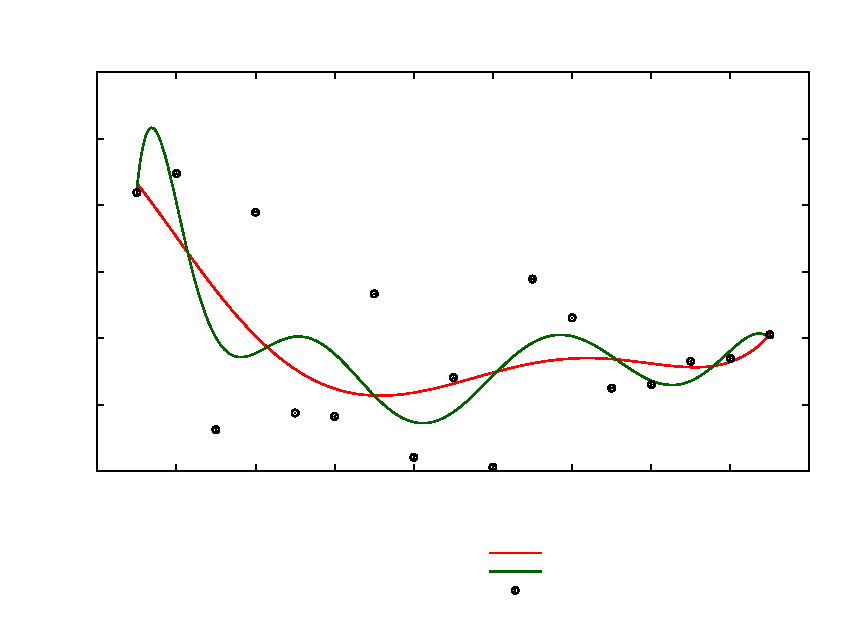
\includegraphics{./../LaTeX/graph/quest1-b}}%
    \gplfronttext
  \end{picture}%
\endgroup

	\caption{Fitting para n = 5, 10}
	\label{fig:quest1-b}	
	\end{subfigure}
	\caption{Gráficos da questão 1}
\end{figure}
\FloatBarrier

\FloatBarrier
\begin{table}
\parbox{.45\linewidth}
		{
		\centering
		\begin{tabular}{|l|l|}\hline
			n & $\alpha_{n}$ \\ \hline
					 0 &  5.449156 \\ \hline 
		 1 &  -1.819039 \\ \hline 
		 1 &  -1.819039 \\ \hline 

		\end{tabular}
		\caption{coeficientes de $y_1(t)$}
		\label{tab:quest1-X1}
		}
\parbox{.45\linewidth}
	{
	\centering
		\begin{tabular}{|l|l|}\hline
			n & $\alpha_{n}$ \\ \hline
					 0 &  8.706067 \\ \hline 
		 1 &  -12.104022 \\ \hline 
		 2 &  5.713879 \\ \hline 
		 2 &  5.713879 \\ \hline 

		\end{tabular}
		\caption{coeficientes de $y_2(t)$}
		\label{tab:quest1-X2}	
	}

\parbox{.45\linewidth}
	{
	\centering
		\begin{tabular}{|l|l|}\hline
			n & $\alpha_{n}$ \\ \hline
					 0 &  11.099895 \\ \hline 
		 1 &  -26.103014 \\ \hline 
		 2 &  24.612518 \\ \hline 
		 3 &  -6.999496 \\ \hline 
		 3 &  -6.999496 \\ \hline 

		\end{tabular}
		\caption{coeficientes de $y_3(t)$}
		\label{tab:quest1-X3}
	}
\parbox{.45\linewidth}
	{
	\centering
		\begin{tabular}{|l|l|}\hline
			n & $\alpha_{n}$ \\ \hline
					 0 &  9.882275 \\ \hline 
		 1 &  -8.734146 \\ \hline 
		 2 &  -44.816147 \\ \hline 
		 3 &  102.115150 \\ \hline 
		 4 &  -72.629829 \\ \hline 
		 5 &  17.150402 \\ \hline 
		 5 &  17.150402 \\ \hline 

		\end{tabular}
		\caption{coeficientes de $y_5(t)$}
		\label{tab:quest1-X5}
	}
	
\parbox{.45\linewidth}
	{
	\centering
		\begin{tabular}{|l|l|}\hline
			n & $\alpha_{n}$ \\ \hline
					 0 &  -41.381470 \\ \hline 
		 1 &  1116.054321 \\ \hline 
		 2 &  -9137.643555 \\ \hline 
		 3 &  37257.980469 \\ \hline 
		 4 &  -87894.031250 \\ \hline 
		 5 &  128680.648438 \\ \hline 
		 6 &  -120650.898438 \\ \hline 
		 7 &  72604.195312 \\ \hline 
		 8 &  -27166.693359 \\ \hline 
		 9 &  5766.708008 \\ \hline 
		 10 &  -532.068542 \\ \hline 
		 10 &  -532.068542 \\ \hline 

		\end{tabular}
		\caption{coeficientes de $y_{10}(t)$}
		\label{tab:quest1-X10}
	}

\end{table}
\FloatBarrier

